\message{ !name(detectors.tex)}
\message{ !name(detectors.tex) !offset(-2) }
%Introduce the NOvA detectors

The original design of the NOvA experiment is laid out in the technical
design report (TDR) \cite{TDR}. The constructed experiment
differs only slightly with the vision laid out in the TDR.

\section{The NuMI Beam}

The NOvA experiment's neutrino source is provided by the Neutrinos at
the Main Injector (NuMI) beam at Fermilab.

%Paragraph in notes form. Revisit!
The produce of the NuMI beam is presented in Figure~\ref{fig:NuMI}.
Protons accelerated up to 120~GeV by the Main Injector. Six batches,
each spanning 10~$\mu sec$. The protons are directed to collide with a
graphite target to create mesons, mostly pions some kaons. 
The mesons
decay producing predominantly muon neutrinos and muons. rock absorber
used to get rid of muons. left with clean beam of muon neutrinos with a
small electron neutrino background.

The focussing horns are used to create a beam of predominantly muon
neutrino or muon anti-neutrino.

% NuMI beam figure
\begin{figure}[!ht]
  \centering
  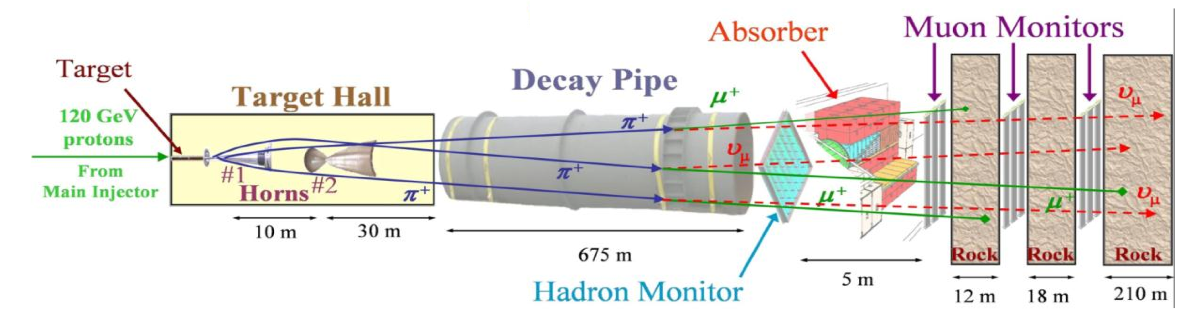
\includegraphics[width=1\textwidth]{../../img/beam/beam_diagram.png}
  \caption{A diagram showing the layout of the NuMI beam}
  \label{fig:NuMI}
\end{figure}





\section{The Near Detector}

\section{The Far Detector}
\message{ !name(detectors.tex) !offset(-42) }
